\chapter{The Hyperbolic Case: The Strata \texorpdfstring{$(2;1^4,2^2;\emptyset)$}{(2;1^4,2^2;empty)}, \texorpdfstring{$(4;1^6;\emptyset)$}{(4;1^6;empty)}, and \texorpdfstring{$(2;1^6;4)$}{(2;1^6;4)} on the Disk}\label{chap:stratoriented}

\section{Introduction}

In this chapter, we analyze the specific strata of pseudo-Anosov homeomorphisms on the 6-marked disk defined by the singularity data $(2; 1^4, 2^2; \emptyset)$, $(4; 1^6; \emptyset)$, and $(2; 1^6; 4)$. We aim to rigorously eliminate these cases by proving the following result:

\begin{theorem}
    \label{thm:orientable_strata_elimination}
    Let $K \subset S^3$ be a hyperbolic knot satisfying $\widehat{HFK}(K) \cong \widehat{HFK}(T_{2,3} \# T_{2,3})$, and let 
    \[
    (h, \phi_h, \hat{h}, \hat{\phi}_h, b, \phi_b, \beta, \phi_\beta, \Phi, \phi_\Phi)
    \]
    be the associated Birman-Hilden correspondence data induced by the monodromy of $K$. Furthermore, let 
    \[
    (\beta, \phi_\beta, \tau, f_\beta)
    \]
    be the geometric data associated with the disk braid, where $\tau$ is a standard train track. Then the pseudo-Anosov representative $\phi_\beta \colon D^2 \to D^2$ (and consequently the invariant train track $\tau$) cannot belong to the strata $(2; 1^4, 2^2; \emptyset)$, $(4; 1^6; \emptyset)$, or $(2; 1^6; 4)$.
\end{theorem}

To achieve this, our primary objective is to establish that the invariant foliations associated with the lifted pseudo-Anosov map on the genus-two surface with two boundary components ($\Sigma_2^2$) in these strata are orientable. This immediately implies that the original monodromy of $K$ also possesses orientable invariant foliations.

Establishing orientability allows us to invoke the homological arguments utilized by Baldwin, Hu, and Sivek \sidecite{baldwin2025khovanov} for their detection result on the cinquefoil. Specifically, once orientability is shown, we apply a theorem of Thurston \sidecite{Thurston1988}, as reformulated by Baldwin-Hu-Sivek, to identify the dilatation $\lambda$ of the pseudo-Anosov map with the spectral radius of its action on the first homology of the branched cover. This action is completely determined by the Alexander polynomial of the knot $K$. We will demonstrate that for $T_{2,3} \# T_{2,3}$, the Alexander polynomial possesses no real roots $\lambda > 1$. This leads to a strict algebraic contradiction, thereby proving that the knot cannot support a pseudo-Anosov monodromy associated with these specific strata.

\section{Orientability of Train Tracks}

We begin by examining the combinatorial structure of the train tracks carrying the pseudo-Anosov maps in the specified strata. Let $\phi_\beta: D^2 \to D^2$ be a pseudo-Anosov homeomorphism of the 6-marked disk, and let $\tau$ be a train track carrying $\phi_\beta$. Note that by Theorem \ref{theorem:theorem C jointless}, we may assume $\tau$ is a jointless standard train track.

Let $\tilde{\tau}$ denote the lift of $\tau$ to the double branched cover $\Sigma_2^2$. As described in Section \ref{sec:lifting train tracks}, $\tilde{\tau}$ carries the lifted mapping class $\Phi$ with pseudo-Anosov representative $\phi_\Phi$. The lifted train track $\tilde{\tau}$ can be viewed geometrically as two copies of the planar train track $\tau$, connected via the lifts of the marked points. 

In the planar track $\tau$, the marked points reside in the interior of infinitesimal polygons. Upon lifting to the double cover, these marked points lift to the Weierstrass points of the hyperelliptic surface. Each of these Weierstrass points is enclosed by infinitesimal polygons obtained by the smoothing procedure described in Section \ref{sec:lifting train tracks}. In the specific strata under consideration, the marked points on the disk are enclosed by either monogons (1-pronged) or bigons (2-pronged). 

Because the covering map acts locally as $w = z^2$, these infinitesimal polygons at the branch locus lift to regions with exactly double the number of sides. The bigons lift to 4-gons. The monogons lift to bigons, which are subsequently smoothed into regular points on the track (eliminating the cusps entirely). Similarly, on the boundary of the lift, the peripheral regions—which are 2-gons and 4-gons on the disk—lift to 4-gons and 8-gons, respectively. Finally, for the stratum $(2; 1^6; 4)$, the un-marked 4-pronged singularity (4-gon) lies in the unbranched interior of the disk; thus, it lifts cleanly to two distinct 4-gons on $\Sigma_2^2$ which are swapped by the hyperelliptic involution.

An equivalent description of the correspondence between $\tau$ and $\tilde{\tau}$ is as follows. Consider the disk $D^2$ embedded in $\mathbb{C}$, with the marked points positioned on the real line. By assumption, $\tau$ is standard, hence only a single side-swapping edge passes vertically above each marked point. We may isotope $\tau$ so that every edge except for the side-swapping edges lies in the upper half-plane; hence the intersection of the underlying graph of $\tau$ with the lower half-plane is a union of disjoint arcs. We can then construct $\tilde{\tau}$ by taking the mirror image of this upper-half-plane graph across the real line and applying the required smoothing procedure at the marked points. This symmetric union is exactly the underlying graph of $\tilde{\tau}$.

\begin{lemma}
\label{lem:even_sided_polygons}
In the strata $(2; 1^4, 2^2; \emptyset)$, $(4; 1^6; \emptyset)$, and $(2; 1^6; 4)$ on $D^2$, every complementary region of the lifted invariant train track $\tilde{\tau}$ on $\Sigma_2^2$ is an even-sided polygon.
\end{lemma}
\begin{proof}
By Proposition \ref{prop:B-H train track polygon enclosure}, the complementary regions of $\tau$ on the disk correspond to the singularities of the foliation. 
\begin{itemize}
    \item In the stratum $(2; 1^4, 2^2; \emptyset)$, the complementary regions are 1-gons, 2-gons, and a peripheral 2-gon. 
    \item In $(4; 1^6; \emptyset)$, they are 1-gons and a peripheral 4-gon. 
    \item In $(2; 1^6; 4)$, they are 1-gons, an interior 4-gon, and a peripheral 2-gon.
\end{itemize}
Since the double branched covering doubles the cone angle at the branch points and the boundary, the 1-gons smooth into 0-gons (regular lines), while the peripheral 2-gons and 4-gons lift strictly to 4-gons and 8-gons on $\Sigma_2^2$. The interior 4-gon in the unbranched region simply lifts to two distinct 4-gons. Therefore, all surviving complementary regions in $\tilde{\tau}$ have an even number of sides.
\end{proof}

We now establish a procedure to specify an orientation for the invariant foliations on $\Sigma_2^2$ by orienting the train track itself.

\begin{definition}[Consistent Orientation]
    Let $\tau$ be a train track. We call an orientation of the real edges of $\tau$ \textbf{consistent} if for every switch $v$ of $\tau$:
    \begin{itemize}
        \item Any two edges forming a cusp at $v$ are both oriented into, or both oriented out of, $v$.
        \item If two incident edges form a valid smooth train path through $v$, they must be oriented so that the train path flows continuously (one entering $v$, one leaving $v$).
    \end{itemize}
\end{definition}

It is immediately clear from this definition that any train track possessing odd-sided polygons (such as monogons or triangles) cannot be consistently oriented. Every polygon has cusps as its corners. Choosing an orientation for an edge incident to a polygon forces orientations on all adjacent edges along the boundary of that region. Since the orientation must flow either strictly into or strictly out of a cusp, it forces an alternating sequence of orientations at each subsequent cusp along the polygon. A cusp whose edges point inward must be adjacent to a cusp whose edges point outward. Consequently, a polygon with an odd number of corners yields an alternating parity contradiction and cannot admit a consistent orientation. 

Conversely, this alternating property ensures that a train track whose complementary regions are strictly even-sided can always be consistently oriented. Topologically, because all regions are even-sided, the complementary regions can be properly 2-colored (analogous to a checkerboard), allowing a globally consistent flow to be assigned to the edges separating them.

\begin{figure}[h]
    \centering
    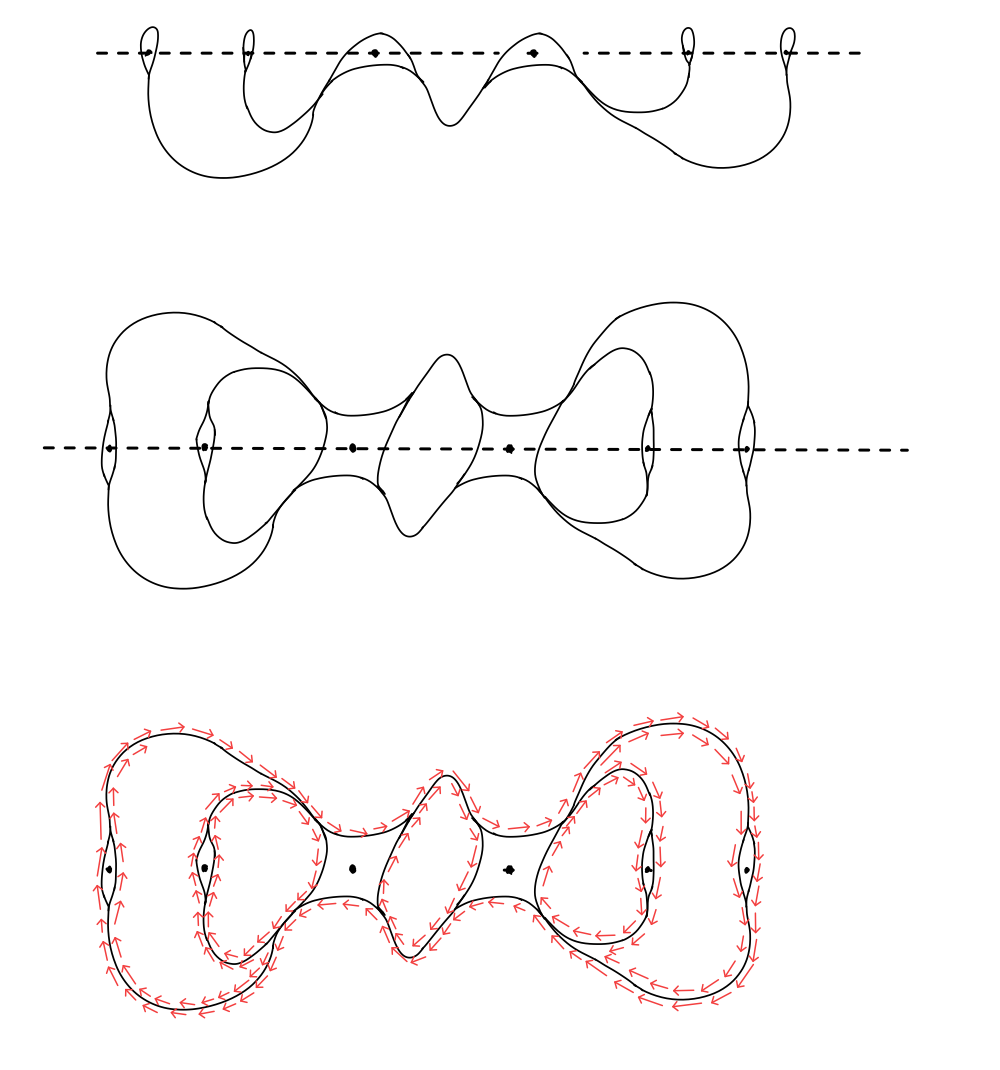
\includegraphics[width=\linewidth]{figures/orienting_traintrack.png}
    \caption[Consistent orientation of a lifted track]{Top: A train track $\tau$ in the stratum $(2;1^4,2^2;\emptyset)$. Middle: Reflecting $\tau$ across the dotted real line and resolving the polygons to produce the lift $\tilde{\tau}$. Bottom: A consistent orientation on $\tilde{\tau}$, possible only because all regions are even-sided.}
    \label{fig:placeholder}
\end{figure}

\begin{prop}
\label{prop:orientable_foliations}
The invariant foliations of a pseudo-Anosov map $\phi_\beta$ belonging to the strata $(2; 1^4, 2^2; \emptyset)$, $(4; 1^6; \emptyset)$, and $(2; 1^6; 4)$ are orientable upon lifting to $\Sigma_2^2$.
\end{prop}

\begin{proof}
Orientability of the foliation on $\Sigma_2^2$ corresponds directly to the existence of a consistent orientation of the edges of the lifted train track $\tilde{\tau}$. By Lemma \ref{lem:even_sided_polygons}, every complementary region in $\tilde{\tau}$ is an even-sided polygon. Because the regions are strictly even-sided and the surface $\Sigma_2^2$ is orientable, the regions can be bipartite colored, which guarantees that a locally consistent choice of edge orientations propagates to a globally consistent orientation of $\tilde{\tau}$.

Considering $\tilde{\tau}$ as embedded in $\Sigma_2^2$, the interior of every $2k$-sided infinitesimal polygon is foliated by the unstable foliation $\mathcal{F}^u$ as described in Section \ref{sec:train track and foliations}. Specifically, the well-defined tangent line at each cusp is parallel to a leaf extending to the interior singularity, forming the $2k$ prongs at the singularity. These separatrices can be oriented in direct accordance with the consistent orientation of the bounding track edges. This partitions the region into $2k$ sectors, each foliated by leaves parallel to the corresponding side. We orient these subregions smoothly in accordance with the consistent orientation of the polygon. This procedure extends the orientation across every interior region of each infinitesimal polygon without contradiction. See Figure \ref{fig:orient_foliation}.

It remains to show that the peripheral regions can be oriented in a compatible way. This is an identical procedure, except that the edges forming the periphery consist of both real edges and portions of the boundary components $\partial_z, \partial_p$. There are $2r$ cusps forming the corners of the peripheral region. The tangent line at each cusp is parallel to a leaf extending to the boundary components, forming the $r$ prongs at each of the two boundary components. These leaves can be oriented in accordance with the locally consistent orientation of the cusps. Because $\tilde{\tau}$ is globally consistently oriented, these paths connect without orientation clashes. We orient the foliations on the surrounding disk by extending the orientation of these paths smoothly towards the boundary. Thus, $\mathcal{F}^u$ is globally orientable.
\end{proof} 

\begin{figure}[h]
    \centering
    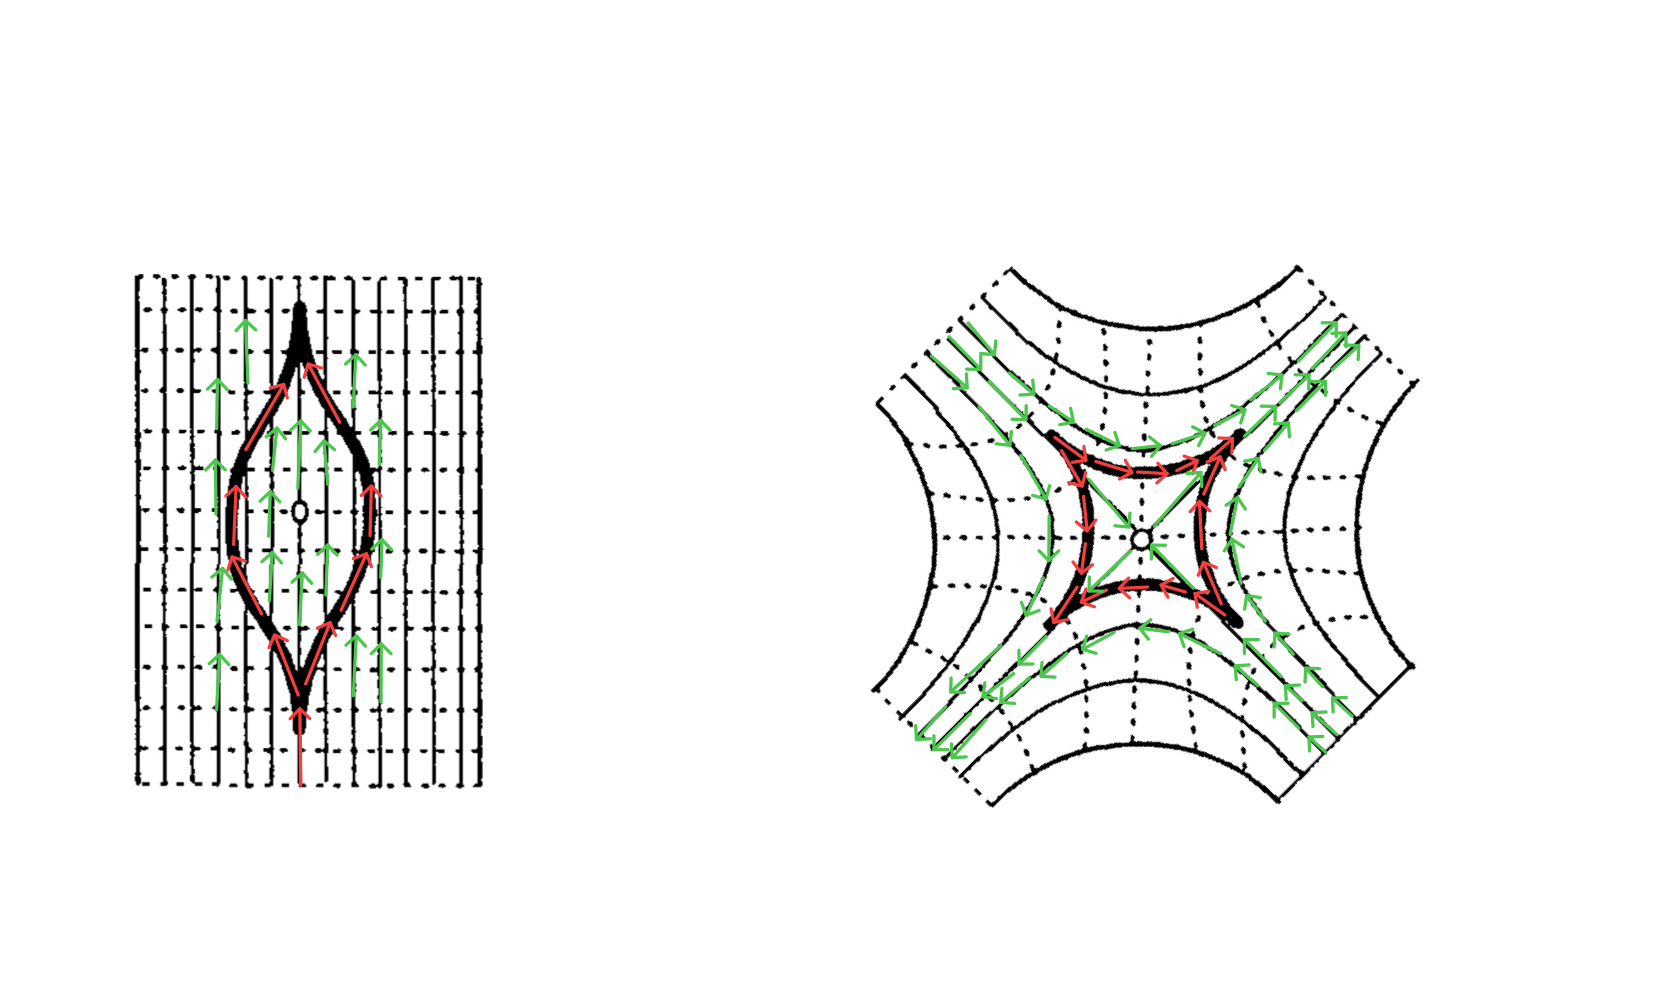
\includegraphics[width=\linewidth]{figures/orient_foliation.png}
    \caption[Inducing foliation orientation from a train track]{Near a singularity, a consistent orientation of the surrounding train track (red arrows) induces a globally consistent orientation on the leaves of the unstable foliation (green arrows).}
    \label{fig:orient_foliation}
\end{figure}

\begin{corollary}
\label{cor:orientable_knot_monodromy}
    Let $K$ be a hyperbolic knot such that $\widehat{HFK}(K) \cong \widehat{HFK}(T_{2,3} \# T_{2,3})$, and suppose 
    \[
    (h, \phi_h, \hat{h}, \hat{\phi}_h, b, \phi_b, \beta, \phi_\beta, \Phi, \phi_\Phi)
    \]
    is the corresponding Birman-Hilden correspondence data. If the disk map $\phi_\beta \colon D^2 \to D^2$ belongs to the strata $(2; 1^4, 2^2; \emptyset)$, $(4; 1^6; \emptyset)$, or $(2; 1^6; 4)$, then the invariant foliations of the original monodromy $\phi_h$ are orientable.
\end{corollary}
\begin{proof}
    By Proposition \ref{prop:orientable_foliations}, the invariant foliations of the fixed-point-free lift $\phi_\Phi$ on $\Sigma_2^2$ are orientable. To recover the invariant foliations of the original knot monodromy $\phi_h$ on $\Sigma_2^1$, we collapse the blown-up boundary component $\partial_z$ back into the interior fixed point $z$, and identify the remaining boundary component $\partial_p$ with the boundary of the knot exterior. Since this local collapse of a boundary curve to a point does not affect the global transverse orientation of the regular leaves, the orientability of the foliation is preserved.
\end{proof}

Having established that the pseudo-Anosov representative $\phi_h$ in these strata must have orientable invariant foliations, we can now strictly relate its dilatation to the homological invariants of the knot. We employ the argument formalized by Baldwin, Hu, and Sivek \cite{baldwin2025khovanov}, in which the dilatation $\lambda(\phi_h)$ manifests as an eigenvalue of the action of the map on the first homology.

\begin{theorem}[Thurston \cite{Thurston1988}; see also {\cite[Theorem~2.2]{LT11}}]
\label{thm:thurston_spectral_radius}
If a pseudo-Anosov homeomorphism $\phi$ on a surface $\Sigma$ preserves an orientable foliation, then its dilatation $\lambda > 1$ is the largest absolute value of a real eigenvalue of the induced map on homology:
\begin{equation}
\lambda = \max \{ |x| : x \in \mathbb{R}, \det(xI - \phi_*) = 0 \},
\end{equation}
where $\phi_* : H_1(\Sigma; \mathbb{R}) \to H_1(\Sigma; \mathbb{R})$.
\end{theorem}

In the context of the monodromy of a knot, the map $\phi = \phi_h$ is the geometric representative of $h$, the monodromy of the fibration associated with the knot $K$. Consequently, the characteristic polynomial of the homological action $\phi_*$ is identified exactly with the Alexander polynomial of the knot.

\begin{corollary}
\label{cor:alexander_root}
For a fibered knot $K$, if the monodromy $\phi_h$ lies in a stratum with orientable invariant foliations, then the dilatation $\lambda(\phi_h)$ must be the largest absolute value of a real root of the Alexander polynomial $\Delta_K(t)$. 
\end{corollary}

\section{Application to \texorpdfstring{$T_{2,3} \# T_{2,3}$}{T(2,3) \# T(2,3)}}

We now apply this algebraic restriction to our specific case: the candidate knot $K = T_{2,3} \# T_{2,3}$. We investigate whether a pseudo-Anosov map in the strata $(2; 1^4, 2^2; \emptyset)$, $(4; 1^6; \emptyset)$, or $(2; 1^6; 4)$ can represent the monodromy of $K$.

The Alexander polynomial for the right-handed trefoil $T_{2,3}$ is given by $\Delta_{T_{2,3}}(t) = t^2 - t + 1$. The Alexander polynomial of the connect-sum is the product of the individual polynomials:
\begin{equation}
\Delta_{K}(t) = \Delta_{T_{2,3}}(t) \cdot \Delta_{T_{2,3}}(t) = (t^2 - t + 1)^2.
\end{equation}

We examine the roots of this polynomial. The roots of $t^2 - t + 1 = 0$ are the primitive sixth roots of unity:
\begin{equation}
t = \frac{1 \pm i\sqrt{3}}{2} = e^{\pm i\pi/3}.
\end{equation}
These roots are strictly complex; they have non-zero imaginary components.

\begin{prop}
\label{prop:no_real_roots}
The polynomial $\Delta_K(t) = (t^2 - t + 1)^2$ has no real roots.
\end{prop}

\begin{proof}
The discriminant of the quadratic factor $t^2 - t + 1$ is $\Delta = (-1)^2 - 4(1)(1) = -3 < 0$. Thus, all roots come in complex conjugate pairs, and none are real.
\end{proof}

\section{Conclusion}

We now assemble the preceding results to formally prove our main theorem.

\begin{proof}[Proof of Theorem \ref{thm:orientable_strata_elimination}]
Assume, for the sake of contradiction, that the knot $K$ admits a monodromy $\phi_h$ corresponding to a disk map $\phi_\beta$ belonging to the strata $(2; 1^4, 2^2; \emptyset)$, $(4; 1^6; \emptyset)$, or $(2; 1^6; 4)$. By Proposition \ref{prop:orientable_foliations}, the invariant foliations of the lifted map $\phi_\Phi$ on $\Sigma_2^2$ are orientable. Because collapsing the blown-up boundary component $\partial_z$ back into the original fixed point $z$ preserves the global transverse orientation of the leaves, the invariant foliations of the original knot monodromy $\phi_h$ on $\Sigma_2^1$ must also be orientable, as established in Corollary \ref{cor:orientable_knot_monodromy}. 

Therefore, by Corollary \ref{cor:alexander_root}, the dilatation $\lambda(\phi_h)$ must be a real root of the Alexander polynomial $\Delta_K(t)$. However, as established in Proposition \ref{prop:no_real_roots}, $\Delta_K(t)$ possesses strictly complex roots and no real roots. Since, by geometric definition, the dilatation of a pseudo-Anosov map must satisfy $\lambda > 1$ (and thus be strictly real), we arrive at a contradiction.

Thus, no pseudo-Anosov representative for the knot $K$ exists within these orientable strata.
\end{proof}

% This elimination constitutes a critical step in the classification of the fiber surface monodromy, demonstrating that Heegaard Floer homology severely restricts the topological dynamics of the knot, systematically reducing the possible pseudo-Anosov strata we must consider.